\documentclass[a4paper, 12pt]{article}
\usepackage{polski}
\usepackage[utf8]{inputenc}
\usepackage[T1]{fontenc}
\usepackage{geometry}
\usepackage{indentfirst}
\usepackage{titlesec}
\usepackage{amsmath}
\usepackage{graphicx}
\usepackage{float}
\usepackage{amssymb}
\usepackage[style=numeric,sorting=none]{biblatex}
\addbibresource{bibliography.bib}


\geometry{top=2.5cm, bottom=2.5cm, left=2.5cm, right=2.5cm}

% Dostosowanie odstępów dla sekcji i podsekcji
\titleformat{\section}[block]{\normalfont\Large\bfseries}{\thesection}{1em}{}
\titlespacing*{\section}{0pt}{3em}{2em} % Odstęp przed i po sekcji
\titleformat{\subsection}[block]{\normalfont\large\bfseries}{\thesubsection}{1em}{}
\titlespacing*{\subsection}{0pt}{2em}{1em} % Odstęp przed i po podsekcji

\begin{document}

    \thispagestyle{empty}

    \begin{center}
        \textbf{\LARGE Politechnika Wrocławska} \\[1em]
        \Large Wydział Matematyki \\[2em]

        \textbf{KIERUNEK:} \\
        \Large Matematyka Stosowana \\[2em]

        \textbf{\LARGE PRACA DYPLOMOWA \\[0.5em] INŻYNIERSKA} \\[6em]

        \textbf{\large TYTUŁ PRACY:} \\[1em]
        \textbf{\Large Analiza efektywności metod uczenia przez wzmacnianie w grach komputerowych} \\[2em]

        \textbf{\large AUTOR:} \\[1em]
        \textbf{\Large Adrian Galik} \\[2em]

        \textbf{\large PROMOTOR:} \\[1em]
        \textbf{\Large dr hab. Janusz Szwabiński } \\[10em]

        WROCŁAW 2024
    \end{center}

    \newpage
    \section{Wstęp}
    W ostatnich dekadach obserwuje się dynamiczny rozwój technologii, który przekracza pierwotne oczekiwania specjalistów.
    Zwiększona dostępność mocy obliczeniowej spowodowała, że algorytmy uczenia maszynowego stały się nieodłączną częścią codziennej aktywności.
    Zastosowania tych algorytmów można odnaleźć w robotyce, rozpoznawaniu obrazów, przetwarzaniu języka naturalnego, klasyfikacji spamu, systemach nawigacyjnych, diagnostyce chorób czy w sztucznej inteligencji dedykowanej grom komputerowym. 
    Każda z wymienionych dziedzin oddziałuje na społeczeństwo zarówno pośrednio, jak i bezpośrednio.
    \\
    \indent Jedną z najciekawszych, a zarazem najdłużej rozwijanych poddziedzin uczenia maszynowego jest uczenie przez wzmacnianie. 
    Metody tego typu, znane już od lat 50. ubiegłego wieku, stanowią centralny punkt rozważań niniejszej pracy.
    \\
    \indent Celem poniższej pracy inżynierskiej jest zbadanie efektywności wybranych metod uczenia przez wzmacnianie w grach komputerowych. 
    Analiza skupia się w szczególności na porównaniu popularnych algorytmów pod kątem czasu uczenia oraz osiąganych wyników.
    W eksperymentach wykorzystano klasyczną grę Pong, często stosowaną w roli środowiska testowego do oceny zachowania agentów sztucznej inteligencji. 
    Zaimplementowano dwie powszechnie używane metody: Deep Q-Learning (DQN), zaproponowaną przez Mnhia et al. \cite{mnih2015dqn}, Advantage Actor-Critic (A2C),
    będącą uporoszczoną wersją asynchronicznych metod aktor-krytyk zaprezentowanych przez Mniha et al. \cite{mnih2016a3c} 
    W kolejnych rozdziałach przedstawiono charakterystykę badanych algorytmów, omówiono przebieg eksperymentu oraz przeanalizowano otrzymane rezultaty.

    \section{Wprowadzenie do uczenia maszynowego}
    Uczenie maszynowe jest jedną z najważniejszych gałęzi sztucznej inteligencji.
    Jego istotę stanowi tworzenie algorytmów zdolnych do samodzielnego nabywania wiedzy na podstawie przetwarzanych danych, bez konieczności programowania konkretnych reguł. 
    Według klasycznej definicji Arthura Samuela z 1959 roku, uczenie maszynowe to „dziedzina nauki dająca komputerom możliwość uczenia się bez konieczności ich jawnego programowania” \cite{samuel1959checkers}.
    Z kolei Tom Mitchell (1997) zwraca uwagę, że „program komputerowy uczy się na podstawie doświadczenia E w odniesieniu do zadania T i pewnej miary wydajności P, jeśli wydajność tego programu (mierzona za pomocą P) wobec zadania T poprawia się wraz z kolejnymi doświadczeniami E” \cite{mitchell1997machinelearning}.
    \\ 
    \indent W praktyce uczenie maszynowe opiera się na zbiorze danych uczących (ang. training set), którego elementy określa się mianem próbek lub przykładów uczących. 
    Modelem zaś nazywa się część systemu odpowiedzialną za wyciąganie wniosków, w oparciu o dostarczone dane oraz proces uczenia. 
    Przykładami modeli mogą być między innymi sieci neuronowe czy lasy losowe.
    \\
    \indent W przypadku zagadnienia klasyfikacji spamu, zadanie T polega na rozróżnianiu, czy dana wiadomość e-mail powinna zostać zakwalifikowana jako „spam” czy „nie spam”. 
    Doświadczeniem E jest tutaj zbiór wiadomości z odpowiednimi etykietami, a miarą wydajności P może być odsetek poprawnie zaklasyfikowanych wiadomości \cite{HandsOnMachineLearning}.
    
    \subsection{Podział uczenia maszynowego}
    Istnieje kilka kategorii uczenia maszynowego, wyróżnianych w zależności od rodzaju dostępnych danych i celu analizy. Najczęściej spotykanymi są:
    
    \subsubsection{Uczenie nadzorowane}
    Uczenie nadzorowane zakłada wykorzystanie zbioru danych z oznaczonymi przez człowieka etykietami. Metoda ta jest szeroko stosowana w zadaniach klasyfikacji (np. klasyfikacja spamu) oraz regresji (np. przewidywanie wartości liczbowych). Do popularnych algorytmów należą między innymi: regresja liniowa, drzewa decyzyjne oraz maszyny wektorów nośnych (SVM).

    \subsubsection{Uczenie nienadzorowane}
    W uczeniu nienadzorowanym algorytm otrzymuje dane bez dodatkowych etykiet, a celem jest odnajdywanie ukrytych wzorców i struktur. Główne zadania obejmują wizualizację danych, redukcję wymiarowości, analizę skupień (klastrów) oraz wykrywanie anomalii. Do typowych algorytmów zaliczają się K-Means oraz DBSCAN.

    \subsubsection{Uczenie częściowo nadzorowane}
    Uczenie częściowo nadzorowane stanowi wariant podejścia nadzorowanego, w którym etykiety nie są nadane ręcznie, lecz automatycznie wyznaczane na podstawie określonych heurystyk lub dodatkowych algorytmów. Metoda ta znajduje zastosowanie w sytuacjach, gdy proces ręcznego oznaczania danych jest kosztowny bądź czasochłonny, co często ma miejsce w diagnozach medycznych.

    \subsubsection{Uczenie przez wzmacnianie}
    Uczenie przez wzmacnianie (ang. reinforcement learning) było przez długi czas mniej popularne niż inne formy, jednak nabrało rozpędu dzięki sukcesom autorów projektu Google DeepMind \cite{mnih2015nature}, którzy zaprezentowali jego skuteczność w grach Atari. Charakteryzuje się tym, że algorytm (zwany agentem) uczy się optymalnych akcji poprzez interakcję z dynamicznym środowiskiem. Po wykonaniu każdej akcji agent otrzymuje nagrodę lub karę, co umożliwia stopniowe dopasowywanie strategii działania w celu maksymalizacji długoterminowego zysku. W ramach niniejszej pracy analizie zostały poddane właśnie takie algorytmy, z naciskiem na ich zastosowanie w środowisku gry Pong.
    \\ \\ 
    Podział uczenia maszynowego na te cztery kategorie jest szeroko akceptowany w literaturze i szczegółowo opisany w \cite{sutton2018rl}.

    
    \section{Teoretyczne podstawy uczenia przez wzmacnianie}

    \subsection{Podstawowe pojęcia i definicje}
    W tej części pracy zastosowano standardowe oznaczenia i definicje stosowane w literaturze dotyczącej uczenia przez wzmacnianie. 
    W szczególności terminologia i symbole (np. \( s, a, r_t, \pi \)) \cite{lapan2020deep}
    \begin{itemize}
        \item \textbf{Agent} - Element systemu wchodzący w interakcje ze środowiskiem poprzez wykonywanie akcji (decyzji) oraz obserwowanie konsekwencji w postaci nagród i stanów.
        Głównym celem agenta jest maksymalizacja długoterminowej nagrody. 
        Przykładowo w szachach agentem może być gracz lub program komputerowy.
        \item \textbf{Środowisko} - Otoczenie, z którym agent ma styczność. 
        Wymiana informacji ze środowiskiem obejmuje jedynie obserwacje (stany) i nagrody.
        Dla gry w szachy środowiskiem jest plansza szachowa wraz z aktualnym układem figur.
        \item \textbf{Stan (\( s \))} - Informacje które środowisko dostarcza agentowi. Dają one wiadomości na temat tego co dzieje się wokół niego.
        \item \textbf{Akcje (\( a \))} - Wszystkie czynności, które agent może podjąć w danym środowisku. 
        Przykładową akcją w szachach jest przesunięcie pionka o jedno pole do przodu.
        \item \textbf{Nagroda (\( r_t \))} - Informacja zwrotna otrzymywana od środowiska, wskazująca na korzystność (bądź niekorzystność) podjętej akcji. 
        Nagroda ma z reguły charakter lokalny, czyli dotyczy wyłącznie niedawno wykonanej akcji, a nie całej historii działań agenta. 
        Zadanie agenta polega na maksymalizacji skumulowanej nagrody w dłuższej perspektywie.
        \item \textbf{Polityka (\( \pi \))} - Strategia agenta, która pomaga mu podejmować akcje w danych stanach. Polityka może być deterministyczna
        (\( \pi(s) = a \)) albo stochastyczna (\( \pi(a|s) \))
    \end{itemize}
    \begin{figure}[H]
        \centering
        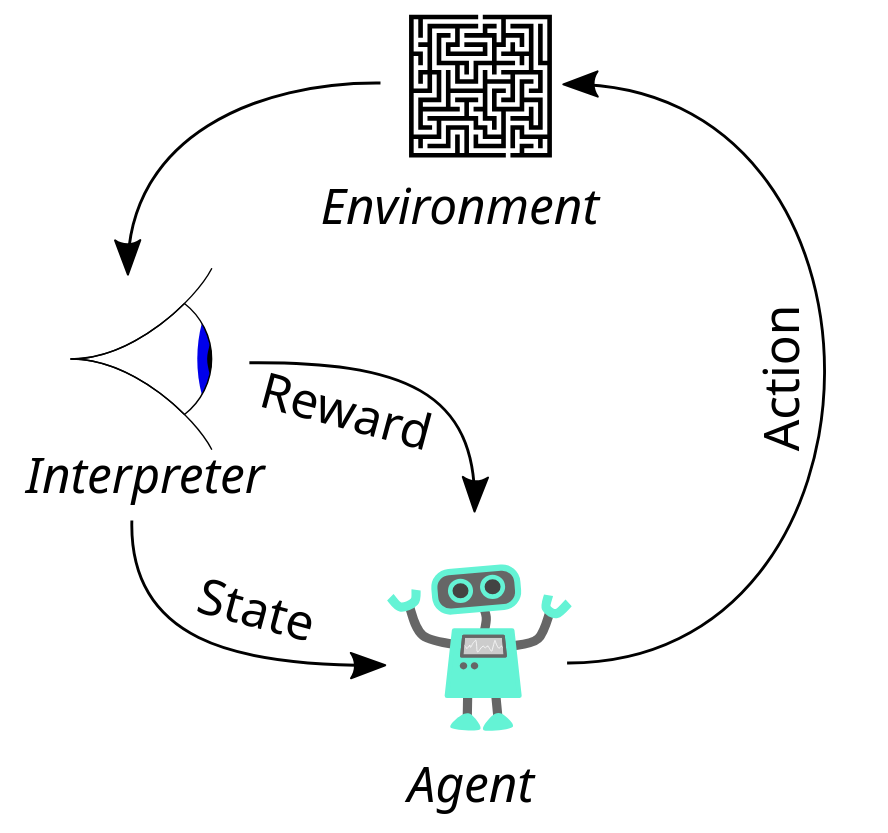
\includegraphics[width=\textwidth]{pictures/Reinforcement_learning_diagram.png}
        \caption{Typowa struktura scenariusza uczenia przez wzmacnianie \cite{wikipedia_reinforcement_learning}}
    \end{figure}

    \subsection{Modele Markowa (MDP)}
    Wzory i definicje użyte w tej sekcji zostały zaczerpnięte z książki „Reinforcement Learning: An Introduction” autorstwa Suttona i Barto \cite{sutton2018rl}.
    Markowskie procesy decyzyjne (MDP) są formalizacją problemów decyzyjnych w warunkach niepewności, które zakładają spełnienie własności markowskiej: przyszłość (kolejny stan i otrzymana nagroda) zależy jedynie od bieżącego stanu i akcji, a nie od pełnej historii.
    W modelu MDP kluczowymi elementami są:
    \begin{itemize}
        \item Stany i akcje - Agent w chwili \( t \) obserwuje stan \( S_t \) ze zbiorów stanów \( S \), a następnie wybiera akcję \( A_t \) z dostępnego zbioru akcji \( A \).
        \item Funkcja przejścia i nagród - Po wykonaniu akcji \( A_t \) w stanie \( S_t \) agent przechodzi do stanu \( S_{t+1} \) i otrzymuje nagrodę \( R_{t+1} \). Oba te elemenety opisuje funkcja:
        \[ p(s',r|s,a) = P(S_{t+1} = s', R_{t+1} = r | S_t = s, A_t = a)\]
        dzięki temu wiadomo z jakim prawdopodobieństwem przy danej akcji w stanie \( s \) agent znajdzie się w stanie \( s' \) oraz jaką otrzyma wtedy nagrodę \( r \).
        \item Oczekiwana nagorda - Bardzo często zamiast śledzić cały rozkład nagród, pracuje się z wartością oczekiwaną natychmiastowej nagrody:
        \[ r(s,a) = E[R_{t+1} | S_t = s, A_t = a] = \sum_{s',r} r p(s',r|s,a)\]
        Innymi słowy, jest to średnia nagroda, jakiej agent może oczekiwać w momencie przejścia ze stanu \( s \) do \( s' \) przy akcji \( a \).
        \item Współczynnik dyskontowania - Aby modelować długofalowe konsekwencje podejmowanych decyzji, wprowadza się współczynnik \( \gamma \in [0,1] \). Określa on, jak silnie agent ceni przyszłe nagrody w porównaniu z bieżącymi. Gdy \( \gamma = 0 \), agent skupia się wyłącznie na nagrodach natychmiastowych, a gdy \( \gamma \) jest bliskie 1, uwzględnia głównie wpływ aktualnej decyzji na dalszą przyszłość.
    \end{itemize}
    \textbf{Skumulowana nagroda} \\ \\ 
    Dla każdego epizodu w uczeniu przez wzmacnianie definiuje się skumulowaną nagrodę w chwili \( t \) następująco:
    \[ G_t = R_{t+1} + \gamma R_{t+2} + ... = \sum_{k=0}^{\infty} \gamma^k R_{t+k+1} \]
    Gdzie:
    \begin{itemize}
        \item \( G_t \) - całkowita (skumulowana) wartość nagród, którą agent otrzymuje od chwili \( t \) aż do zakończenia epizodu,
        \item \( \gamma \) - współczynnik dyskontowania z przedziału \( [0,1] \), który wyznacza, jak bardzo agent ceni przyszłe nagrody w stosunku do natychmiastowych,
        Na przykład:
        \begin{itemize}
            \item Dla \( \gamma = 0 \), agent skupia się wyłącznie na nagrodach natychmiastowych,
            \item Gdy \( \gamma \) jest blisko 1, agent korzysta z długoterminowych strategii co może przyniać się do bardziej sensownych akcji,
        \end{itemize}
        \item \( R_{t+k+1} \) - Nagroda otrzymana przez agenta w kroku czasowym \( t + k + 1 \). Są to nagrody będące sygnałami zwrotnymi otrzymanymi
        od środowiska, mające na celu informowanie agenta o jakości jego działań,
        \item \( k \) - indeks czasowy który określa zasięg możliwości przyszłych decyzji agenta, dzięki któremu jest w stanie obliczyć skumulowaną nagrodę.
        Sumowanie zaczyna się od \( k = 0 \) co wskazuje nagrodzie otrzymanej po wykonaniu akcji w stanie \( S_t \).
    \end{itemize}
    Skumulowana nagroda \( G_t \) jest ma kluczowe znaczenie w uczeniu przez wzmacnianie ponieważ określa ocenę jakości działań agenta. Stanowi ona podstawyw cel, który agent stara się 
    maksymalizować poprzez optymalny wybór akcji.
    \\ \\ 
    \textbf{Funkcje wartości i algorytmy uczenia}
    \begin{itemize}
        \item Funckja wartości stanu \( V_\pi(s) \) - Oczekiwana skumulowana nagroda przy założeniu, że agent znajduje się w stanie \( s \) i przestrzega polityki \( \pi \):
        \[ V_\pi(s) = E_\pi[G_t|S_t=s] \]
        \item Funkcja wartości akcji \( Q_\pi(s,a) \) - Oczekiwana skumulowana nagroda przy wykonaniu akcji \( a \) w stanie \( s \), a następnie kontynuacji zgodnie z polityką \( \pi \):
        a następnie postępując zgodnie z polityką \( \pi \).
        \[ Q_\pi(s,a) = E_\pi[G_t|S_t=s,A_t=a] \]
    \end{itemize}
    Funkcje te są kluczowe w wielu algorytmach uczenia przez wzmacnianie. 
    W podejściu Q-learning następuje iteracyjna aktualizacja wartości \( Q \) w celu wyznaczenia optymalnej polityki,
    natomiast w metodach typu aktor-krytyk (np. A2C) równocześnie modyfikuje się politykę (aktor) i funkcję wartości (krytyk).
    \\ \\ 
    \textbf{Przykład dla gry Pong}
    \\ \\ 
    W celu zilustrowania pojęcia skumulowanej nagrody można rozważyć epizod w grze Pong, gdzie agent otrzymuje w kolejnych krokach czasowych następujące nagrody:    \begin{itemize}
        \item \( r_1 = +1 \) (zdobycie punktu)
        \item \( r_2 = -1 \) (utrata punktu)
        \item \( r_3 = +1 \)
        \item \( r_4 = +1 \)
        \item \( r_5 = -1 \)
    \end{itemize}
    Zakładając że \( \gamma = 0.9 \), wtedy skumulowana nagroda \( G_0 \) zaczynając od chwili \( t = 0 \) będzie obliczana jako:
    \[ G_0 = \gamma^0r_1 + \gamma^1r_2 + \gamma^2r_3 + \gamma^3r_4 + \gamma^4r_5 + ... \]
    \[ G_0 = 1 * 1 + 0.9 * (-1) + 0.9^2 * 1 + 0.9^3 * 1 + 0.9^4 * (-1) + ... \]
    \[ G_0 = 1 - 0.9 + 0.81 + 0.729 - 0.6561 + ... \]
    Maksymalizacja tej sumy wymusza na agencie podejmowanie decyzji zapewniających możliwie największy zysk nie tylko w bieżącym kroku, lecz także w dalszych etapach rozgrywki.
    \subsection{Równanie Bellmana}
    Wzory i definicje użyte w tej sekcji zostały zaczerpnięte z książki „Reinforcement Learning: An Introduction” autorstwa Suttona i Barto \cite{sutton2018rl}.
    Równanie Bellmana pełni kluczową rolę w teorii uczenia przez wzmacnianie, umożliwiając sformalizowanie zależności między wartościami stanów a podejmowanymi akcjami.
    Używane jest głównie do iteracyjnego obliczania wartości funkcji stanów i akcji, co stanowi fundament wielu algorytmów. 
    Jak zauważyli Sutton i Barto (2018), Równanie Bellmana stanowi podstawę dla większości algorytmów uczenia przez wzmacnianie, ponieważ pozwala na efektywne obliczanie wartości stanów i akcji poprzez iteracyjne aktualizacje \cite{sutton2018rl}.
    \subsubsection{Równanie Bellmana dla funkcji wartości stanu \( V_\pi(s) \)}
    Funkcja wartości stanu \( V_\pi(s) \) wyraża oczekiwaną sumę zdyskontowanych nagród, jakie agent może uzyskać, rozpoczynając od stanu \( s \) i postępując zgodnie z polityką \( \pi \). 
    Równanie Bellmana w tym kontekście ma postać:
    \[ V_\pi(s) = E_\pi[R_{t+1} + \gamma G_{t+1}|S_t = s] = \sum_{a} \pi(a|s) \sum_{s',r} p(s',r|s,a) (r + \gamma V_\pi(s')) \],
    gdzie:
    \begin{itemize}
        \item \( V_\pi(s) \) - Funckja stanu wartości dla polityki \( \pi \), określająca sumę zdyskontowanych nagród od stanu \( s \),
        \item \( E_\pi \) - wartość oczekiwana względem rozkładu wyznaczonego przez politykę \( \pi \),
        \item \( R_{t+1} \) - nagroda otrzymywana po przejściu do stanu \( S_{t+1} \) w wyniku podjęcia akcji zgodnej z \( \pi \), 
        \item \( \gamma \) - Współczynnik dyskonotwania z przedziału \( [0,1] \),
        \item \( S_{t+1} \) - Stan osiągnięty po wykonaniu akcji w stanie \( s \).
    \end{itemize}
    Równanie to można interpretować poprzez równość wartości stanu s a oczekiwanej nagrodzie otrzymanej po przejściu do kolejnego stanu plus zdyskontowanej wartości nowego stanu,
    zakładając, iż agent działa zgodnie z polityką \( \pi \).
    \subsubsection{Równanie Bellmana dla funkcji wartości akcji \( Q_\pi(s,a) \)}
    Funkcja wartości akcji \( Q_\pi(s,a) \) reprezentuje oczekiwaną sumę zdyskontowanych nagród, uzyskiwanych przez agenta w sytuacji, gdy w stanie ss podjęta zostanie akcja \( a \), a w kolejnych krokach zastosowana zostanie polityka \( \pi \). Odpowiednie równanie Bellmana ma postać:
    \[ Q_\pi(s,a) = E_\pi[R_{t+1} + \gamma G_{t+1}|S_t = s, A_t = a] = \sum_{a} \pi(a|s) \sum_{s',r} p(s',r|s,a)(r + \gamma \sum_{a} \pi(a|s)Q_\pi(s',a')) \]
    Zgodnie z tym równaniem wartość akcji \( a \) w stanie \( s \) zależy od natychmiastowej nagrody oraz zdyskontowanej wartości przyszłych akcji, które zostaną wybrane zgodnie z polityką \( \pi \).
    \subsubsection{Równanie Bellmana dla polityki optymalnej \( V_*(s) \) i \( Q_*(s,a) \)}
    Polityka optymalna \( \pi_* \) maksymalizuje funkcję wartości stanu. Oznacza to, że:
    \[ V_*(s) = \max_{\pi} V_{\pi}(s), \]
    Równanie Bellmana dla optymalnej funkcji wartości stanu może zostać zapisane w postaci:
    \[ V_*(s) = \max_{a} E[R_{t+1} + \gamma V_*(S_{t+1})|S_t = s, A_t = a] = 
    \max_{a} \sum_{s',r} p(s',r|s,a)(r + \gamma V_*(s'))\]
    Analogicznie, optymalna funkcja wartości akcji wyraża się wzorem:
    \[ Q_*(s,a) = E[R_{t+1} + \gamma \max_{a'} Q_*(S_{t+1},a')|S_t = s, A_t = a] =
    \sum_{s',r} p(s',r|s,a)(r + \gamma \max_{a'} Q_*(s',a')) \]
    Powyższe równania można interpretować następująco:
    \begin{itemize}
        \item \( V_*(s) \) - Najlepsza możliwa wastość stanu \( s \), uzyskana poprzez wybór najlepszej akcji.
        \item \( Q_*(s,a) \) - Najlepsza możliwa wartość akcji \( a \) w stanie \( s \), przy założeniu dalszego postępowania według optymalnych decyzji.
    \end{itemize}
    Opisane zależności leżą u podstaw algorytmów takich jak Value Iteration czy Q-learning, które dążą do znalezienia polityki maksymalizującej skumulowaną nagrodę.
    \subsubsection{Metoda iteracji wartości}
    Algorytm, który pozwala na uteracyjną aktualizację funkcji wartości stanu \( V(s) \) zgodnie z rówaniem Bellmana dla optymalnej polityki, do momentu osiągnięcia zbieżności.
    \\ Składa się ona z poniższych kroków:
    \begin{itemize}
        \item Zainicjalizuj wszystkie stany \( V_i \) z pewnymi wartościami początkowymi. Zawyczaj \( V(s) = 0 \) dla wszystkich \( s \in S \).
        \item Dla każdego stanu \( s \in S \) w procesie decyzyjnym Markowa wykonaj aktualizacje:
        \[ V(s) \leftarrow \max_a \sum_{s',r} p(s',r|s,a)[r + \gamma V(s')] \]
        \item Powtarzaj poprzedni krok poprzez wykonanie wielu iteracji do momentu gdy maksymalna zmiana \( V(s) \) jest mniejsza niż zadany próg. 
    \end{itemize}
    \subsubsection{Metoda iteracji polityki}
    Algorytm składający się z dwóch głównych kroków: ewaluacji polityki i jej ulepszania. Składa się on z poniższych kroków:
    \begin{itemize} 
        \item Zainicjalizuj początkową politykę \( \pi(s) \) oraz \( V(s) \)
        \item Oblicz wartość \( V(s) \) dla bierzącej polityki \( \pi \) za pomocą poniższego wzoru:
        \[ V(s) \leftarrow \sum_{s',r} p(s',r|s,\pi(s))(r + \gamma V(s'))\]
        \item ulepszenie polityki poprzez wybór akcji \( a \) maksymalizującej wartość oczekiwaną dla każdego stanu \( s \) za pomocą poniższego wzoru:
        \[ \pi'(s) = argmax_a \sum_{s',r} p(s',r|s,a) [r + \gamma V(s')] \]
        \item Jeżeli \( \pi' = \pi \), kończy się proces w przeciwnym wypadku ustaw \( \pi \leftarrow \pi' \) i ponów kroki 2-3.
    \end{itemize}
    \subsection{Metoda entropii krzyżowej w uczeniu przez wzmacnianie}
    Wzory i definicje użyte w tej sekcji zostały zaczerpnięte z książki „Deep Reinforcement Learning Hands-On.” autorstwa Maxima Lapana \cite{lapan2020deep}.
    Entropia krzyżowa jest miarą różnicy pomiędzy dwoma rozkładami prawdopodobieństwa. W kontekście uczenia przez wzmacnianie bywa wykorzystywana do oceny jakości nowej polityki \( \pi_{new} (a|s) \) względem idealnego rozkładu akcji, który ma maksymalizować skumulowaną nagrodę. Definicja entropii krzyżowej pomiędzy rozkładami \( p(a) \) i \( q(a) \) ma postać:
    \[ H(p,q) = - \sum_{a \in A} p(a) log(q(a)) \]
    gdzie:
    \begin{itemize}
        \item \( p(a) \) - Jest rozkładem prawdopodobieństwa akcji \( a \) według starej polityki \( \pi_{old}(a|s) \).
        \item \( q(a) \) - Jest rozkładem prawdopodobieństwa akcji \( a \) według nowej polityki \( \pi_{new} (a|s) \).
    \end{itemize} 
    \subsubsection{Twierdzenie o próbkowaniu istotnościowym}
    Próbkowanie istotnościowe pozwala na wykorzystanie próbek pochodzących z pewnego rozkładu prawdopodobieństwa w celu oszacowania wartości oczekiwanej funkcji definiowanej względem innego rozkładu. W uczeniu przez wzmacnianie z próbkowaniem istotnościowym ma się do czynienia np. wtedy, gdy dane są zbierane na podstawie starej polityki \( \pi_{old}(a|s) \), zaś celem jest szacowanie wartości dla nowej polityki \( \pi_{new} (a|s) \). Zgodnie z twierdzeniem:
    \\ Twierdzenie o próbkowaniu istotnościowym:
    \[ E_{x \sim p(x)} [H(x)] = \int_{x} p(x)H(x) dx = \int_{x} q(x) \frac{p(x)}{q(x)} H(x) dx = E_{x \sim q(x)} [\frac{p(x)}{q(x)}H(x)]\] 
    gdzie:
    \begin{itemize}
        \item \( p(x) \) - Rozkład próbkowania (np. stara polityka)
        \item \( q(x) \) - Rozkład docelowy (np. nowa polityka)
        \item \( H(x) \) - Funkcja entropi w stanie \( x \) często definiowana jako:
        \[ H(\pi) = - \sum_{a \in A} \pi(a|s)log(\pi(a|s)) \]
    \end{itemize}
    \subsubsection{Dywergencja Kullbacka-Leiblera}
    Dywergencja Kullbacka-Leiblera (KL) mierzy odległość między dwoma rozkładami prawdopodobieństwa \( p(x) \) i \( q(x) \). W uczeniu przez wzmacnianie może służyć do kontrolowania, jak bardzo nowa polityka różni się od starej, co pomaga zapobiegać gwałtownym zmianom w trakcie treningu. Definicję KL przedstawia równanie:
    \[ KL(p(x) || q(x)) = \sum_{x} p(x) \frac{p(x)}{q(x)}\]
    W kontekście uczenia przez wzmacnianie:
    \[ KL(\pi_{old}(a|s) || \pi_{new}(a|s)) = \sum_{a} \pi_{old}(a|s) log(\frac{\pi_{old}(a|s)}{\pi_{new}(a|s)})\]
    Dywergencja Kullbacka-Leiblera w kontekście uczenia przez wzmacnianie jest używana do:
    \begin{itemize}
        \item Regularizacji polityki - Ogranicza stopień smiany między starą a nową polityką, co pomaga uniknąć niestabilnych lub niepożądanych zachowań podczas trenowania,
        \item Kontrola eksploracji - Wspiera utrzymanie równowagi między eksploracją nowych akcji a wykorzystywaniem już poznanych strategii.
    \end{itemize}
    \section{Implementacjia wybranych algorytmów uczenia przez wzmacnianie}
    W dziedzinie uczenia przez wzmacnianie istnieje szeroki zakres różnych algorytmów, a ich wybór w dużej mierze
    jest zależny od środowiska w jakim algorytmowi przyszło pracować. algorytmy te można podzielić na trzy główne kategorie:
    \begin{itemize}
        \item Algorytmy optymalizujące wartości (Value Optimization)
        \item Algorytmy optymalizujące politykę (Policy Optimization)
        \item Algorytmy imitacyjne (imitation)
    \end{itemize}
    \subsection{Klasyfikacja algorytmów uczenia przez wzmacnianie}
    \subsubsection{Algorytmy optymalizujące wartości (Value optimization)}
    Algorytmy tej kategorii są skoncentrowane na nauce funkcji wartości, która ma za zadanie ocenić jakość stanów lub akcji w danym czasie.
    Najbardziej znanym algorytmem tej kategorii jest \textbf{Q-Learning}, który ma nacelu nauke funkcji \textbf{\( Q(s,a) \)}, 
    która reprezentuje oczekiwaną sumę zdyskontowanych nagród po wykonaniu akcji \( a \) w stanie \( s \) oraz postępuje ona zgodnie z optymalną polityką.
    \\ \textbf{Przykłady algorytmów:}
    \begin{itemize}
        \item Q-Learning
        \item Deep Q-Learning (DQN)
        \item double DQN
        \item dueling DQN
    \end{itemize}
    \subsubsection{Algorytmy optymalizujące politkę (Policy Optimization)}
    Algorytmy te działają na zasadzie bezpośredniej optymalizacji polityki agenta, czyli regułę wyboru akcji w każdym stanie.
    Algorytm zamiast uczyć się funkcji wartości, optymalizuje politkę starając się znaleść najbardziej korzystną politykę na zasadzie maksymalizacji
    oczekiwanej sumy nagród.
    \\ \textbf{Przykłady algorytmów:}
    \begin{itemize}
        \item Policy Gradient Methods (REINFORCE)
        \item Advantage Actor-Critic (A2C)
        \item Asynchronous Adbantage Actor-Critic (A3C)
        \item Proximal Policy Optimization (PPO)
    \end{itemize}
    \subsubsection{Algorytmy imitacyjne (imitation)}
    Algorytmy imitacyjne naśladują działania eksperta dzięki czemu uczą się jak poprawnie się zachowywać. Celem jest
    stworzenie odpowiedniej polityki, która ma na celu reprodukcje sukcesów eksperta bez konieczności eksploracji środowiska.
    \\ \textbf{Przykłady algorytmów:}
    \begin{itemize}
        \item Behavioral Cloning
        \item Inverse Reinforcement Learning (IRL)
        \item Generative Adversarial Imitation Learning (GAIL)
    \end{itemize}
    \subsection{Wybór algorytmów do implementacji}
    W kontekście realizacji mojego projektu zdecydowałem się na implementacji algorytmów należących do dwóch z pierwszych kategorii a mianowicie:
    \textbf{Deep Q-Learning (DQN)}, \textbf{Advantage Actor-Critic (A2C)} oraz \textbf{Asynchronous Advantage Actor-Critic (A3C)}.
    Za podjęciem tej decyzji w dużej mierze odpowiadało wybrane środowisko i specyfikacja zadania.
    \subsubsection{Dlaczego odrzucono klasyczną metodę Q-Learning?}
    Klasyczna metoda uczenia przez wzmacnianie jaką jest Q-Learning chodź stanowi fundament, posiada dość spore ograniczenia co 
    czyni ją nieskuteczną w bardziej złożonych środowiskaj, takich jak gry wideo. Z głównych powodów które doprowadziły 
    do zrezygnowania z metody Q-Learning w tym projekcie są:
    \begin{itemize}
        \item Wysoka wymiarowość przestrzeni stanów - Gry takie jak Pong, ale także inne gry z kategori gier Atari generują bardzo złożone 
        i wysoko wymiarowe dane wejściowe, przez co ze względu na bardzo dużą ilość pamięci do przechowywania wartości \( Q(s,a) \),
        tablicowe podejście algorytmu Q-Learning staje się niepraktyczne.
        \item Brak generalizacji - Klasyczna metoda Q-Learning nie jest w stanie generować doświadczeń do nowych, nieznanych stanów, co 
        przyczynia się do sporego ograniczenia efektywnego uczenia się w dynamicznych środowiskach.
        \item Trudność z eksploracją - Wysoki poziom eksploracji który jest wymagany przez Q-Learning doporwadza do sporego czasu oczekiwania.
        \item Brak stabilności procesu uczenia - Model Q-Learning dla dużych przestrzeni stanów oraz dynamicznych środowisk jest niestabilny co prowadzi
        do trundości a nawet niemożliwości osiągnięcia konwergencji modelu. 
    \end{itemize}
    Ze względu na powyższe powody zdeycydowałem się na wykorzystanie bardziej zaawansowanych metod które wykorzystują ogromne zasoby jakie daje im 
    wykorzystanie sieci neuronowych do aproksymacji wartości funkcji.
    \subsection{Deep Q-Learning (DQN)}
    Algorytm Deep Q-Learning (DQN) jest bardziej zaawansowaną metodą od zwykłego Q-Learning gdyż wykorzystuję głębokie sieci neuronowe.
    Została ona zaprojektowana w celu efektywnego radzenia sobie z dużymi i złożonymi przestrzeniami stanów które są trudne a nawet nie możliwe
    do obsłużenia przez tradycyjną metodę Q-Learning. Przy pomocy zastosowania głębokich sieci neuronowych algorytm umożliwia agentom
    uczenie sie w bardziej efektywny sposób zaawansowanych strategii w środowiskach o wysokiej złożoności, takich jak gry wideo.
    \subsubsection{Architektura modelu}
    Architektura modelu Deep Q-Learning opiera się na głębokiej sieci neuronowej, która pełni rolę funkcji aproksymującej 
    Q-funkcję \( Q(s,a;\theta) \). Główne elementy architektóry DQN to:
    \begin{itemize}
        \item Sieć Q (Q-Network):
        \begin{itemize}
            \item Wejście - Stan środowiska \( s \), który może mieć reprezentacje na przerózne sposoby, np: jako wektor cech 
            czy też surowe dane.
            \item Warstwy ukryte - Kilka warst neuronowych często konwolucyjnych w przypadku na przykład przetwarzania obrazów.
            Są one głównie odpowiedzialne za ekstrakcję cech i przetwarzanie informacji z wejścia.
            \item Warstwa wyjściowa - Wyprowadza wartości \( Q \) dla każdej możliwej akcji \( a \) w danym stanie \( s \).
        \end{itemize}
        \item Sieć docelowa (Target Network) - Jest ona kopią sieci \( Q \) mającą na celu aktualizację rzadziej niż sieć \( Q \).
        Sieć docelowa służy do generowania celów dla aktualizacji Q-funkcji, co pomaga w odpowiedniej stabilizacji procesu uczenia.
        \item Bufor doświadczeń (Experience Replay Buffer) - Mechanizm który pozwala na przechowanie przejść (\( s_t, a_t, r_{t+1}, s_{t+1} \)),
        które są później losowo pobierane do treningu. Za pomocą tego agent jest w stanie się uczyć różnorodnych doświadczeń,
        co pozwala mu na redukcje korelacji między kolejnymi próbami i ulepsza stabilizację procesu uczenia.
    \end{itemize}
    \subsubsection{Przykładowa architektura sieci Q dla DQN}
    \begin{itemize}
        \item Warstwa wejściowa - Wejście w postaci obrazu o rozmiarze 84x84 pikseli z 4 kanałami
        \item Pierwsza warstwa konwolucyjna - 32 filtry, rozmiar jądra 8x8, stride 4, aktywacja ReLU.
        \item Druga warstwa konwolucyjna - 64 filtry, rozmiar jądra 4x4, stride 2, aktywacja ReLU.
        \item Trzecia warstwa konwolucyjna - 64 filtry, rozmiar jądra 3x3, stride 1, aktywacja ReLU.
        \item Warstwa w pełni połączona - 512 neuronów, aktywacja ReLU.
        \item Warstwa wyjściowa - Liczbna neronów jest równa liczbie dostępnych akcji w środowisku, bez wykorzystania funkcji aktywacji
    \end{itemize}
    \subsubsection{Proces treningu algorytmu DQN}
    Proces treningu obejmuje kilka kluczowych dla działania etapów mających na celu efektywne uczenie się optymalnej polityki.
    Poniżej jest przedstawiony opis etapów krok po kroku:
    \begin{itemize}
        \item Zainicjalizuj \( Q(s,a;\theta) \) za pomocą początkowego przybliżenia:
        \begin{itemize}
            \item Sieć Q - Zaincjalizowanie parametrów sieci \( Q \) z losowymi wartościami.
            \item Sieć docelowa - Skopiowanie wag sieci \( Q \) do sieci docelowej.
            \item Bufor doświadczeń - Utworzenie pustego bufora do przechowywania przejść (\( s_t, a_t, r_{t+1}, s_{t+1} \)).
        \end{itemize}
        \item Wybór akcji (strategia \( \epsilon \)-greedy): \\
        Agent wybiera kacjię \( a_t \) na podstawię bierzącego stanu \( s_t \) za pomocą strategii \( \epsilon \)-greedy.
        \[
        a_t =
        \begin{cases} 
        \text{Losowa akcja} & \text{z prawdopodobieństwem } \epsilon, \\
        \arg\max_a Q(s_t, a; \theta) & \text{z prawdopodobieństwem } 1 - \epsilon.
        \end{cases}
        \]
        \item Agent wykonuje wybraną akcję \( a_t \) w środowisku, co prowadzi do otrzymania nagrody \( r_{t+1} \)
        oraz przejścia do nowego stanu \( s_{t+1} \)
        \item Przechowanie doświadczenia (\( s_t, a_t, r_{t+1}, s_{t+1} \)) w buforze.
        \item Pobranie mini-partii przejść (\(s_i, a_i, r_i s'_i \)) doświadczeń z bufora
        \item Obliczenie targetów Q-values za pomocą wzoru:
        \[ y_i = r_i + \gamma max_{a'}Q(s'_i,q';\theta^-) \]
        gdzie \( \theta^- \) jest parametrem docelowej sieci
        \item Aktualizacja sieci Q poprzez minimalizację funkcji straty błędu średniokwadratowego (MSE):
        \[ \mathcal{L}(\theta) = \frac{1}{N} \sum_{i}(Q(s_i,a_i;\theta)-y_i)^2 \]
        \item aktualizacja sieci docelowej:
        \[ \theta^- \leftarrow \theta \]
    \end{itemize}
    \subsubsection{Zalety i wady DQN}
    \noindent \textbf{Zalety:}
    \begin{itemize}
        \item Efektywność w dużych przestrzeniach stanów dzięki głębokim sieciom neuronowym
        \item Stabilizacja uczenia za pomocą mechanizmów replay i target network
    \end{itemize}
    \textbf{wady:}
    \begin{itemize}
        \item Terning sieci DQN wymaga znaczących zasobów obliczeniowych
        \item Kluczowe w treningu sieci DQN jest dobranie odpowiednich hiperparametrów dla odpowiedniej optymalizacji
        co może nieść za sobą spore trudności.
        \item Problemy z eksploracją. Model może utknąć w lokalnym minimum.
    \end{itemize}
    \subsection{Advantage Actor-Critic (A2C)}
    Advantage Actor-Critc (A2C) to metoda, która łączy w sobie zalety metod opartych na polityce i opartych na wartściach.
    Pozwala ona na zminiejszczenie wariancji poprzez uzależnienie punktu odniesienia od stanu. Nagrodę można przedstawić
    jako wartość stanu plus przewaga akcji: \( Q(s,a) = V(s) + A(s,a) \). A2C działa na zasadzie wykorzystania dwóch odzielnych
    sieci nauronowych: aktora odpowiedzialnego za wybur akcji oraz krytka oceniającego jakość wypranych akcji.
    \subsubsection{Architektura modelu}
    Aktor jest odpowiedzialny za generowanie rozkładu prawdopodobieństwa akcji \( \pi(a|s) \)
    w danym stanie 
    \begin{itemize}
        \item Warstwa wejściowa która przyjmuje stan środowiska \( s_t \) jako wejście. Stan ten może być representowany jako wektor cech lub inna odpowiednia reprezentacja.
        \item Warstwy ukryte reprezentowane jako kilka warstw neuronowych w pełni połączonych lub konwolucyjnych które
        mają za zadanie przetworzyć informacje z wejścia
        \item Warstwa wyjściowa która używa funkcji softmax w celu wyprowadzenia rozkładu prawdopodobieństwa akcji:
        \[ \pi(a|s) = \frac{exp(f(a,s))}{\sum_{a'}exp(f(a',s))} \]
        gdzie \( f(a,s) \) jest wynikiem ostatniej warstwy sieci aktora.
    \end{itemize}
    krytyk ocenia wartość stanu \( V(s) \) oraz przewagi akcji \( A(s,a) \) w danym stanie, co jest kluczowe dla podejmowania odpowiednich akcji przez aktora.
    \begin{itemize}
        \item Warstwa wejściowa przyjmuje ten sam stan środowiska \( s_t \) co aktor.
        \item Warstwy ukryte są reprezentowane jako kikla warstw neuronowych mających za zadanie przetwarzać informacje z wejścia.
        \item Warstwa wyjściowa ma na celu wyprowadzić jendą wartość funckji skalarnej wartości stanu:
        \[ V(s) = f(s) \]
        gdzie \( f(s) \) jest wynikiem ostatniej warstwy sieci krytyka.
    \end{itemize}
    Warto także wspomnieć o wspóldzieleniu warstw przez algorytm A2C mianowice część warstw sieci może być współdzielona między
    aktorem a krytykiem, co pozwala na efektywniejsze uczenie się współnych reprezentacji stanów.
    \subsubsection{Proces treningu algorytmu A2C}
    Poniższy opis procesu A2C obejmuje interakcje agenta ze środowiskiem, zbieranie doświadczeń, obliczanie przewagi i aktualizację wag sieci aktora i krytyka.
    \begin{itemize}
        \item Inicjalizacja procesu uczenia z parametrami sieciowymi \( \theta \) przyjmując wartrości losowe dla obu sieci aktora i krytyka.
        parametr polityki \( \theta_\pi \) (aktor), parametr wartości \( \theta_v \) (krytyk)
        \item Wykonać \( N \) kroków w środowisku używając bieżącej polityki \( \pi_\theta \). Dla każdego kroku
        \( t \) zapamiętać stan \( s_t \) akcję \( a_t \) wylosowaną z \( \pi_{\theta_\pi} (a|s_t) \), nagrodę \( r_t \).
        \item Jeżeli dotarliśmy do końca epizodu, przyjmujemy \( R = 0 \) w przeciwnym wypadku obliuczamu wartość stanu końcowego \( s_{t+1} \)
        Przy pomocy sieci wartości:
        \[ R = V_{\theta_v}(s_{t+1}). \]
        W przypadku zakończenia epizodu na przykład gdy gra się kończy przerywamy zbieranie danych wcześniej.
        \item Przetwarzamy kroki wstecz od \( t = t_N, t_{N-1}, ..., t_{start} \), obliczając skumulowaną nagrodę z dyskonotwaniem:
        \[ R \leftarrow r_t + \gamma R \]
        następnie należy aktualizować gradnienty aktora i krytyka:
        \begin{itemize}
            \item Gradient polityki:
            \[ \nabla \theta_\pi \leftarrow \nabla \theta_\pi log \pi_{\theta_\pi} (a_t|s_t) (R-V_{\theta_v}(s_t)) \]
            \item Gradient wartości:
            \[ \nabla \theta_v \mathcal{L}_v \leftarrow \frac{\partial}{\partial \theta_v} (R - V_{\theta_v}(s_t))^2 \]
        \end{itemize}
        Sumujemy powyższe gradienty dla aktora i krytyka w pamięci co w praktyce zbiera się je wektorem przez \( N \) kroków.
        \item Zaktualizować parametry sieci wykorzystując zsumowane gradienty. Wektor \( \nabla \theta_\pi \) dodajemy do \( \theta_\pi \) (maksymalizacja polityki) oraz
        wektor \( \nabla \theta_v \) odejmujemy od \( \theta_v \) (minimalizacja błędu wartości).
        \item Powtarzamy procedure z kroku 2 do momentu osiągnięcia konwergencji lub uzyskania założonych winików.
    \end{itemize}
    \subsubsection{Zaleti i wady A2C}
    \noindent \textbf{Zalety:}
    \begin{itemize}
        \item Lączenie zalet metod opartych na polityce i wartości poprzez kożystanie zarówno z optypalizacji polityki, jak i oceny stanu jakości przez krytyka.
        \item Stabilność uczenia się dzięki wykorzystaniu przewagi \( A(s,a) \) oraz regularyzacji entropii.
        \item Efektywna eksploracja poprzez regularyzację entropii.
        \item Skalowalność
    \end{itemize}
    \textbf{Wady:}
    \begin{itemize}
        \item Złożoność obliczeniowa. Algorytm A2C wymaga trenowania dwóch oddzielnych sieci neuronowych dla aktora i krytyka co zwiększa
        wymagania obliczeniowej
        \item Wrażliwość na parametry takie jak cwspółczynnik regulacji entropii \( \beta \), współczynnik dyskonotwania \( \gamma \) 
        oraz współczynnik uczenia \( \alpha \).
        \item Potencjalne problemy z równowagą aktora i krytyka, która przy niewłaściwej synchronizacji może doprowadzić do niestabilnosći w procesie uczenia
    \end{itemize}
    \section{Eksperymenty i analiza wyników}
    \subsection{Konfiguracja środowiska testowego}
    Głównym celem pracy jest przeprowadzenie eksperymentów z uczeniem przez wzmacnianie do prostej gry typu Atari. 
    Ze względu na to zdecydowano się na wybór gry Pong jako środowiska testowego. W celu łatwości implementacji oraz eliminacji
    nadmiarowej ilościu kodu zdecydowano się skorzystać z zasobów biblioteki Gymnasium która zapewnia jednolity
    interfejs API dla agenta uczenia przez wzmacnianie.
    \subsubsection{Środowisk testowe: Pong}
    Pong jest popularną grą wideo z kategorii gier Atari, które idealnie się nadają do testowania algorytmów takich jak uczenie przez wzmacnianie,
    dlatego zdecydowano się na użycie tej gry. Biblioteka Gymnasium (następca biblioteki Gym) oferuje szeroką gamę możliwości testowych poprzez gre Pong.
    Wiele algorytmów zostało przetestowanych i wykorzystanych jako benchmark w uczeniu maszynowych ze względu na prostotę implementacji biblioteki. Warto też zwrócić
    uwagę iż pong wymaga od agenta skutecznego podejmowania decyzji w czasie rzeczywistym co nadaje się idealnie do testów.
    \subsubsection{Charakterystyka środowiska Pong:} 
    \begin{itemize}
        \item Stan Środowiska - Stanem środowiska jest aktualny widok gry który wyświetla obraz, który ma wymiary 210 x 160 x 3 (wysokośc, szerokość, kanały RGB).
        W celu efektywnego uczenia obraz jest przetwarzany wstępnie w celu redukcji wymiarów oraz uproszczenia danych wejściowych
        \item Zbiór akcji - Dla gry Pong mamy możliwość wykonania trzech akcji: przesunięcie paletki w góre, przesunięcie paletki w dół oraz pozostawienie paletki w miejscu.
        \item Nagrody - Sposób przyznawania nagród dla naszego środowiska wyraża się w następujący sposób: +1: Agent zdobywa punkt w momencie odbica piłki w taki sposób aby przeciwnik nie był w stanie jej odbić,
        -1: W momencie gdy agent nie doła odbić piłki przeciwnik otrzymuje punkt, 0: Dla pozostałych przypadków np: w trakcie wymiany odbić.
        \item Warunek końca epizodu - Koniec jednego epizodu uczenia następuje w momencie, gdy agent lub jego przeciwnik osiągnie 21 punktów.
        \item Cel agenta - Głównym zadaniem agenta jest maksymalizacja całkowitej zdyskontowanej nagrody podczas jednego epizodu gry, co oznacza wygrywaniu z przewagą większej ilości punktów niż przeciwnik.
    \end{itemize}
    \subsubsection{Język programowania: Python}
    W ramach implementacji algorytmów uczenia przez wzmacnianie zdecydowano się na użycię języka programowania Python. Głównymi aspektami przemawiającym za wybraniem tego języka są przedewszystkim szeroka
    gama bilbiotek wspierających uczenie przez wzmacnianie np. Gymnasium, Pytorch. Python jest najpopularniejszym językiem sotosowanym w dziedzinie sztucznej inteligencji i uczenia przez wzmacnianie. Duża ilość 
    współczesnych algorytmów sztucznej inteligencji została zaprojektowana przy pomocy Pythona co także skłania do skorzystania z tego języka programowania. 
    \subsubsection{Biblioteki wykorzystane do implementacji}
    \begin{itemize}    
        \item Gymnasium - Biblioteka stanowiąca standard dla uczenia przez wzmacnianie służąca do symulacji środowsik. Zastosowaną ją głównie w celu dostarczenia środowiska gry pong, oraz
        łatwości w zapewnieniu interfejsu dla agenta który ma mu służyć jako interakcja ze środowiskiem. Biblioteka oferuje prostą interakcję z różnymi algorytmami uczenia przez wzmacnianie.
        \item PyTorch - Pozwala na implementacje złożonych modeli uczenia przez wzmacnianie opartych na sieciach neuronowych za pomocą kilku linijek kodu. 
        PyToch zapewnia dwie wysokopoziomowe funkcję: Obliczenia tensorowe z silną akceleracją przy pomocy wykorzystania procesorów graficznych, 
        Wykorzystanie głębokich sieci neuronowych zaprojektowanych za pomocą taśmowych systemów automatycznego różnicowania.
        \item OpenCV - Zestaw narzędzi pozwalający na przetwarzanie obrazu oraz wizję komputerową wizję zadań. Dzięki wykorzystaniu tej biblioteki jesteśmy w stanie
        osiągnąć szybkie iw wydajne przetwarzanie danych wizualizacyjnych przed przesłaniem ich do sieci neuronowej, dzięki czemu uzyskujemy 
        pozytywny efekt w postaci czasu treningu oraz jego efektywności. 
    \end{itemize}
    \subsection{Kryteria oceny modeli}
    \subsection{Wyniki dla modelu Deep Q-Learning}
    Model Deep Q-Learning został zaimplementowany w celu wytrenowania agenta do gry Pong, za pomocą
    wykorzystania głębokich sieci neuronowych w do aproksymacji wartości funkcji Q. Strutura algorytmu opiera się na wykorzystaniu
    bibliotek PyTorch, Gymnasium oraz OpenCV. Środowisko zostało odpowiednio dostosowane za pomocą wrapperów, mających na celu poprawę
    efektywności i jakości danych wejściowych. 
    \newpage
    \subsubsection{Analiza wykresu nagordy}
    \begin{figure}[htbp]
        \centering
        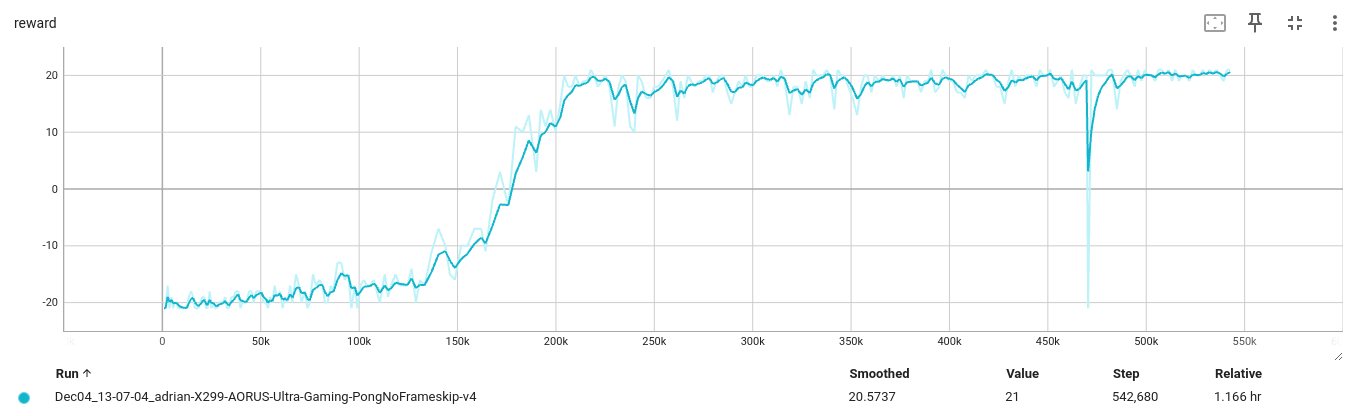
\includegraphics[width=\textwidth]{pictures/DQL_reward.png}
        \caption{Opis obrazka}
        \label{fig:etykieta_obrazka}
    \end{figure}
    Na podstawię poniższego wykresu przedstawiającego proces uczenia modelu Deep Q-Learning widzimy, że na początku treningu agent wykonuje
    losowe ruchy czyli ekspoloruje środowisko, co jest adekwatne do otrzymywania nagród na poziomie około -21 czyli maksymalnej możliwej przegranej. 
    Następnie następuje powolny wzrost wartości nagród co wskazuje na powolne szukanie podstawowych strategii przez agenta. W momencie około 100 000 
    kroków treningowych następuje gwałtowny wzrost otrzymywanej średniej nagrody agenta co wskazuje na stopniową naukę strategii gry.
    W okolicach około 175 000 kroków średnia nagroda zaczyna przekraczać punkt 0 co oznacza iż agent zaczyna wygrywać więcej razy w trakcie jednego epizodu gry.
    W momencie około 300 000 kroków można zaobserwować osiągnięcie stopniowej stablności wyników, zbliżając się do maksymalnej średniej nagrody wynoszącej +21.
    W kolejnych krokach widać niewielkie wachania wyników co jest związane z stochastyczną naturą dynamicznego środowiska gry Pong.
    Proces treningu został zakończony w ciągu około 540 000 kroków, przy czasie trwania procesu uczenia wynoszącym 1,166 godziny czasu rzeczywistego.
    \subsubsection{Opis implementacji modelu Deep Q-Learning}
    Implementacja modelu składa się z następujących elementów:
    \begin{itemize}
        \item Architektura sieci neuronowej - Do modelu DQN wykorzystano seić neuronową która jest głęboką siecią konwolucyjną składającą się z poniższych warstw:
        \begin{itemize}
            \item Warstwy konwolucyjne:
            \begin{itemize}
                \item Pierwsza warstwa: 32 filtry o rozmiarze 8 x 8 i kroku 4.
                \item Druga warstwa: 64 filtry o rozmiarze 4 x 4 i kroku 2.
                \item Trzecia warstwa: 64 filtry o rozmiarze 3 x 3 i kroku 1.
            \end{itemize}
            Celem zastosowania warstw konwolucyjnych jest redukcja wymarowości wejściowego obrazu oraz wyodrębnienie istotnych cech dla podejmowania decyzji przez agenta
            \item Warstwy w pełni połączone:
            \begin{itemize}
                \item jedna warstwa o 512 neuronach z funkcją aktywacji ReLU.
                \item Warstwa wyjściowa odpowiadająca za generacje Q-wartości dla każdej możliwej akcji wykonanej przez agenta.
            \end{itemize}
        \end{itemize}
        \item Przygotowanie danych wejściowych - Do odpowiedniego przetworzenia danych wejściowych zastosowano poniższe wrappery:
        \begin{itemize}
            \item MaxAndSkipEnv
            \item FireResetEnv
            \item ProcessFrame84
            \item ImageToPyTorch
            \item BufferWrapper
            \item ScaledFloatFrame
        \end{itemize}
        \item Mechanizm bufora powtórki (replay buffer) - Służy do przechowywania i próbkowania partii danych podczas treningu. Rozmiar bufora: 10 000 ostatnich doświadczeń.
        Próbkowanie doświadczeń odbywa się poprzes losowe wybieranie 32-elementowych mechanizmów uczenia wsadowego (batch learning) w celu minimalizacji korelacji między próbkami.
        \item Wykorzystanie algorytmu epsilonu zachłannego - Ma na celu stworzenie strategii która pozwala na połączenie akcji eksploracji i eksploatacji. Początkowa wartość epsilonu: 1.0
        (losowe wybory). Stopniowy spadek wartości epsilonu do momentu 0.01 w ciągu 150 000 kroków.
        \item Synchronizacja sieci docelowej - Sieć docelowa zostaje zsysnchronizowana z główną siecią co 1000 kroków w celu poprawy stabilności porcesu uczenia.
    \end{itemize}
    \subsubsection{Problem przetrenowania modelu}
    Podczas testów modelu poprzez wyświetlenie gry Pong w postaci aplikacji można zaobserwować iż modele ze średnim wynikiem 10-21 grają w bardzo specyficzny sposób. Agent mimo wysokiej
    skuteczności w osiąganiu wyników w środowisku Pong, wykonywał ruchu które w zasadzie przewidywały już zachowanie przeciwnika na którym odbywało się trenowanie. Takie zachowanie wskazuje
    na nadmierne dopasowanie do danych treningowych. Ten problem, znany jako przetrenowanie (overfitting), jest szczególnie istotny w algorytmach uczenia przez wzmacnianie.
    \\ \\ \textbf{Przyczyny przetrenowania modelu DQN:}
    \begin{itemize}
        \item Ograniczona różnorodność danych w replay buffer - Replay buffer przechowuje ograniczoną liczbę doświadczeń do 10 000 ostatnich kroków. 
        W momencie gdy agent dominuję daną strategię gry, bufor może być wypełniony głównie przykładami wspierającymi taką startegię, co prowadzi do utraty różnorodności danych.
        W praktyce agent uczy się przewidywania konkretnych scenariuszy, które często występują w buforze, co skutkuje brakiem przygotowania na bardziej niestandardowe sytuacje.
        \item Eksploatacja kosztem eksploracji - Podczas późniejszych etapów uczenia, gdy wartość \( \epsilon \) w strategii epsilon-greedy spada do 0.01, agent w praktyce przestaje 
        eksplorować nowe akcje, korzystając jedynie z wyuczonych optymalnych ruchów. Skutkuje to brakiem otkrywania alternatywnych strategii.
        \item Brak elementu stochastyczności w wyborze akcji - Wybór akcji w modelu DQN dokonuje się na podstawie maksymalizacji wartości \( Q \), co może prowadzić do sztywnego
        dopasowania do konkretnego zestawu stanu i akcji, bez uwzględnienia potencajlnie równie dobrych alternatyw.
        \item Brak mechanizmów zapobiegających przetrenowaniu - Ze względu na swoją naturę model DQN nie uwzględnia mechanizmów regulujących eksplorację (np. entropii polityki)
    \end{itemize}
    \textbf{Zastosowanie Generatywnych Sieci Przeciwstawnych (GAN) jako możliwe rozwiązanie problemu przetrenowania - }
    Jednym z potencjalnych rozwiązań problemu przetrenowania jest zastosowanie generatywnych sieci przeciwstawnych w celu zwiększenia różnorodności danych oraz poprawy modelu.
    To podejście może zostać użyte do tworzenia syntetycznych trajektorii w środowisku gry Pong, które byłyby trudne dla agenta, co zmusiłoby go do bardziej uniwersalnego zachowania.
    Także dzięki temu osiągamy możliwość wprowadzenia stochastyczności w wyborze stanów i akcji, które agent rzadko widzi w trakcie treningu, co zmniejsza ryzyko nadmiernego dopasowania.
    Dzięki bardziej zróżnicowanym doświadczeniom za pomocą zastosowania tego podejścia, agent staje się lepiej przygotowany na nietypowe sytuacje podczas gry. 
    Ze względu na bardzo dużą trudność w implementacji generatywnych sieci przeciwstawnych dla modelu DQN zdecydowano się stworzyć inny model (A2C).
    Także dużym problemem po zastosowaniu tego podejścia jest dostosowanie hiperparametrów, które muszą być dla tego przypadku perfekcyjnie dobrane.
    \subsubsection{Tabela z wynikami dla różnych hiperparametrów}
    \subsubsection{Wnioski}
    Model Deep Q-Learning (DQN) wykazał dużą skuteczność w nauce gry Pong, osiągając maksymalną średnią nagrodę równą +21, co wskazuje na pełne opanowanie środowiska przez agenta.
    Proces uczenia przebiegł zgodnie z założeniami - początkowe wyniki były bardzo niskie, co wynikało z losowej eksploracji środowiska, następnie z biegiem czasu treningu agent stopniowo
    uczył się nowych strategii i popbrawiał swoje wyniki, ąż do momentu osiągniuęcia zauważalnej stabilności w momencie przekroczenia około 300 000 kroków.
    Mechanizm bufora powtórki pozwolił na efektywne przechowywanie i ponowne wykorzystanie doświadczeń, a strategia epslion-greedy przyczyniła sie do balansu między eskploracją 
    nowych akcji a eksploatacją wyuczonych strategii. Mimo sporych sukcesów osiągniętych przez model DQN można zaobserwować pewne ograniczenia, szczególnie w późniejszych etapach treningu.
    Zauważono zjawisko przetrenowania, które objawiało się w postaci nienaturalnych ruchów agenta, które wskazują na nadmierne dopasowanie do danych. Problem ten wynikał w dużej mierze 
    z natury modelu DQN który ma ograniczoną różnorodność danych w buforze oraz malejącą wartość epsilonu, która redukuje eksplorację na korzyść eksploatacji. 
    Ze względu na te problemu postanowiono zastosować bardziej zaawansowany algorytm taki jak A2C, który charakteryzuje się lepszym balansem
    między eksploracją a aksplatacją dzięki polityce stochastycznej. Podsumowujcąc, mimo iż model DQN jest skuteczny w grze Pong, jego ograniczenia
    w zakresie przetrenowania, długioego czasu konwergencji oraz wrażliwości na hiperparametry wskazują na potrzebę zastosowania bardziej zaawansowanych podejść.
    Model ten jest idealnym punktem wyjścia jeśli chodzi o dalsze badania, ale w praktycznych zastosowaniach wymaga dużej ilości wsparcia w postaci dodatkowych 
    mechanizmów usprawniających eksplorację oraz optymalizację.
    \subsection{Wyniki dla modelu Advantage Actor-Critic (A2C)}
    Model Advantage Actor-Critic (A2C) został zaimplementowany z celu poprawy stabilności i efektywności prcesu uczenia w porównaniu do klasycznego algorytmu Deep Q-Learning (DQN).
    Wykorzystuje on równoległe środowiska oraz jednoczesne uczenie polityki i fuynkcji wartości, dzięki czemu agent podejmuje lepsze decyzje. 
    Za pomocą zastosowania regularyzacji entropii, model A2C unika problemu nadmiernego dopasowania, wspierając eksplorację środowiska.
    Poniżej przedstawiono wyniki uzyskane podczas treningu modelu A2C. Wykresy ilustrują kluczowe aspekty procesu uczenia, między innymi: przewaga (\( A(s,a) \)), zmiany funkcji nagrody,
    gradienty oraz straty. Za pomocą tych wizualizacji można przeanalizować szczegółowo zachowanie modelu podczas procesu uczenia oraz ocenić jego efektywność w kontekście rozważanego problemu.\
    \subsubsection{Analiza wykresów dla modelu A2C} 
    \noindent \textbf{Wykres przewagi (\( A(s,a) \))} 
    \begin{figure}[H]
        \centering
        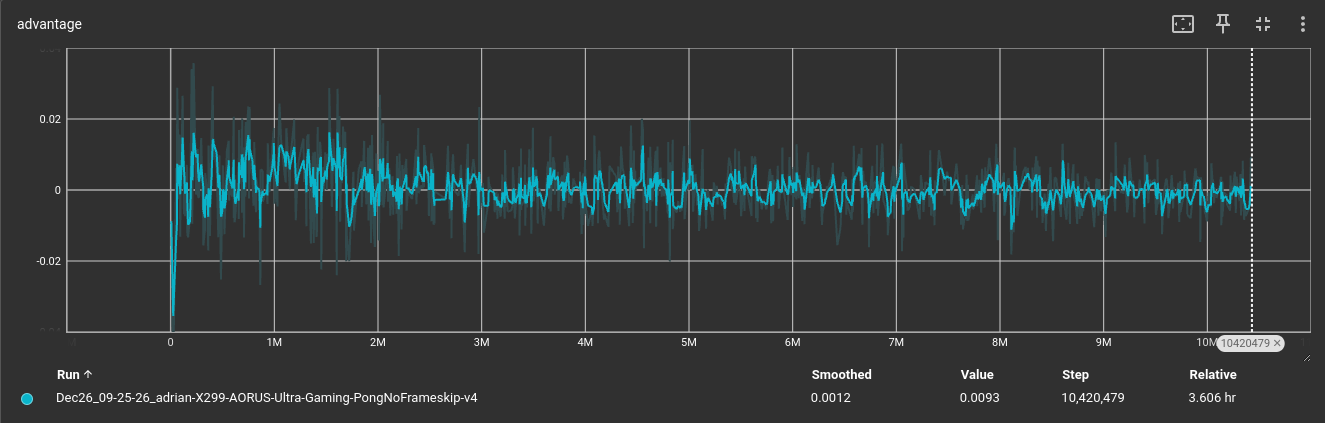
\includegraphics[width=\textwidth]{pictures/A2C_advantage.png}
        \caption{Opis obrazka}
    \end{figure}
    Wykres przedstawia wartość przewagi, czyli rożnice między wartością stanu a wartością oczekiwaną na podstawie polityki, jest to kluczowy element procesu uczenia w modelu A2C.
    Na wykresie można zaobserwować wahania wartości w trakcie treningu, co wskazuje na róznorodność w ocenie podejmowanych decyzji przez agenta.
    Stabilizacja wartości przewagi w późniejszych etapach wskazuje na to, że model zaczyna poprawnie się uczyć podejmowania decyzji oraz optymalizacji polityki.
    \\ \\ 
    \textbf{Wykres średniej wartości paczki}
    \begin{figure}[H]
        \centering
        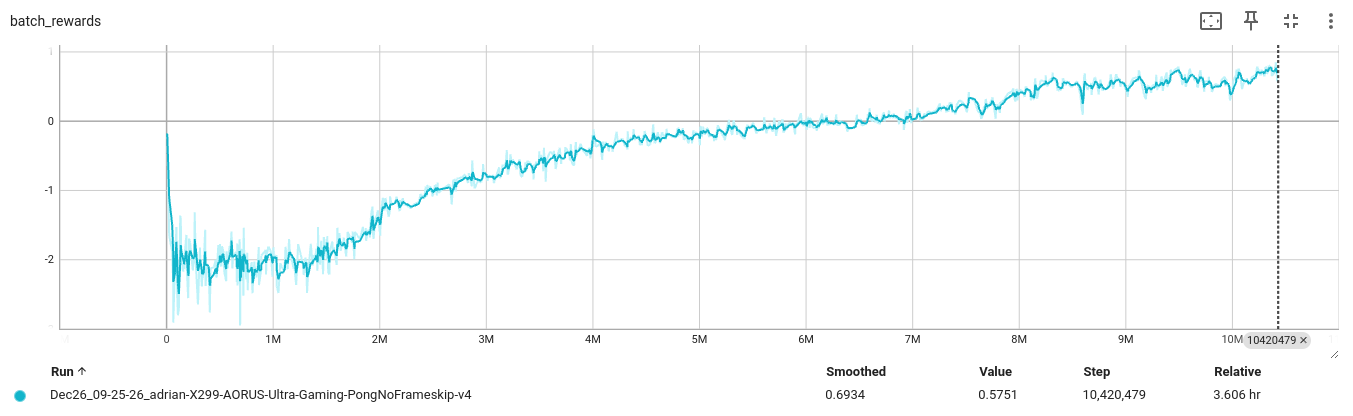
\includegraphics[width=\textwidth]{pictures/A2C_batch_rewards.png}
        \caption{Opis obrazka}
    \end{figure}
    Wykres przedstawia sumaryczne nagrody zebrane przez agenta w kolejnych epizodach.
    Początkowy wzorst wartości wskazuje na adaptację modelu do środowiska.
    W późniejszych etapach zaobserwowano regularny wzrost nagród co sugeruję poprawę strategii agenta, która skutkuje osiąganiem coraz lepszych wyników.
    \\ \\ 
    \textbf{Wykres Normy L2 gradnientu}
    \begin{figure}[H]
        \centering
        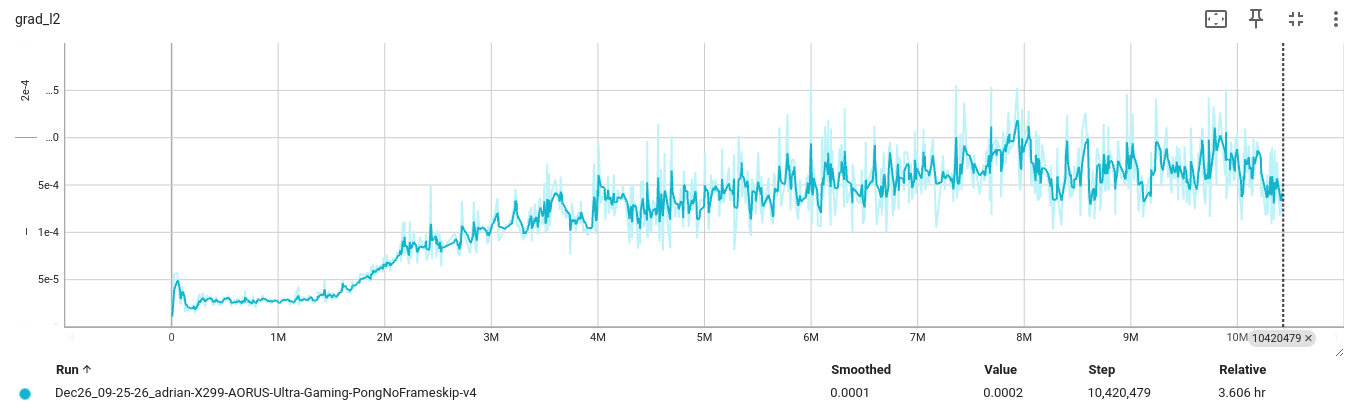
\includegraphics[width=\textwidth]{pictures/A2C_grad_l2.png}
        \caption{Opis obrazka}
    \end{figure}
    Wartość L2-normy gradientów moniotruje siłę aktualizacji parametrów modelu. Zbyt duże wartości gradientów prowadzą do niestabilności procesu uczenia, 
    natomiast zbyt małe prowadzą do problemów z osiągnięciem konwergencji. Uzyskany wykres pokazuje stabilizację norm gradientów podczas treningu,
    co wskazuje na skutceczne zarządzanie porcesem optymalizacji.
    \\ \\ 
    \textbf{Wykres maksymalnych gradientów}
    \begin{figure}[H]
        \centering
        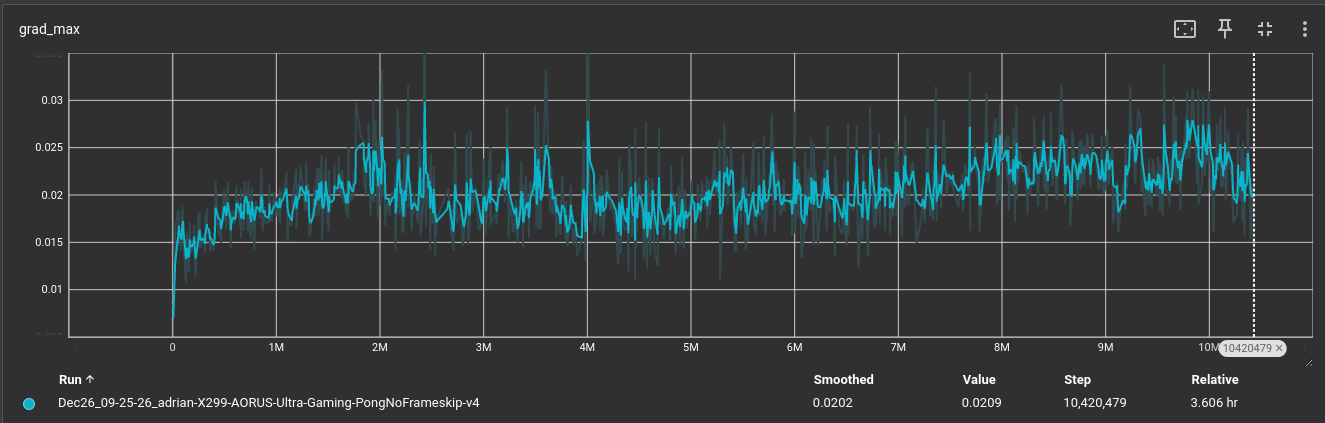
\includegraphics[width=\textwidth]{pictures/A2C_grad_max.png}
        \caption{Opis obrazka}
    \end{figure}
    Maksymalne wartości gradientów wskazują na bardziej znaczące zmiany parametrów podczas trenowania modelu.
    Stabilizacja ich w późniejszym procesie treningu sugeruje, iż model zaczyna osiągać równowagę w uczeniu oraz dostosowywaniu się do środowiska.
    \\ \\ 
    \textbf{Wykres wariancji gradientów}
    \begin{figure}[H]
        \centering
        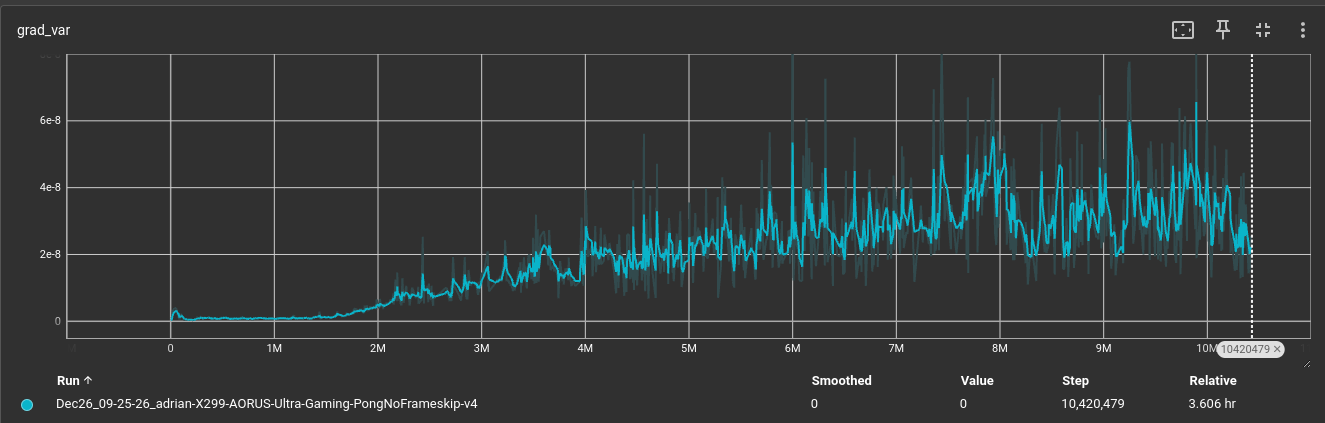
\includegraphics[width=\textwidth]{pictures/A2C_grad_var.png}
        \caption{Opis obrazka}
    \end{figure}
    Wariancja gradientów pokazuje, jak bardzo różnią się gradienty dla różnych partii danych. 
    Na początku procesu uczenia jest ona bardzo mała, ale później zaczyna rosnąć co oznacza, że polityka ulega zmianie.
    \\ \\ 
    \textbf{Wykres straty entropii}
    \begin{figure}[H]
        \centering
        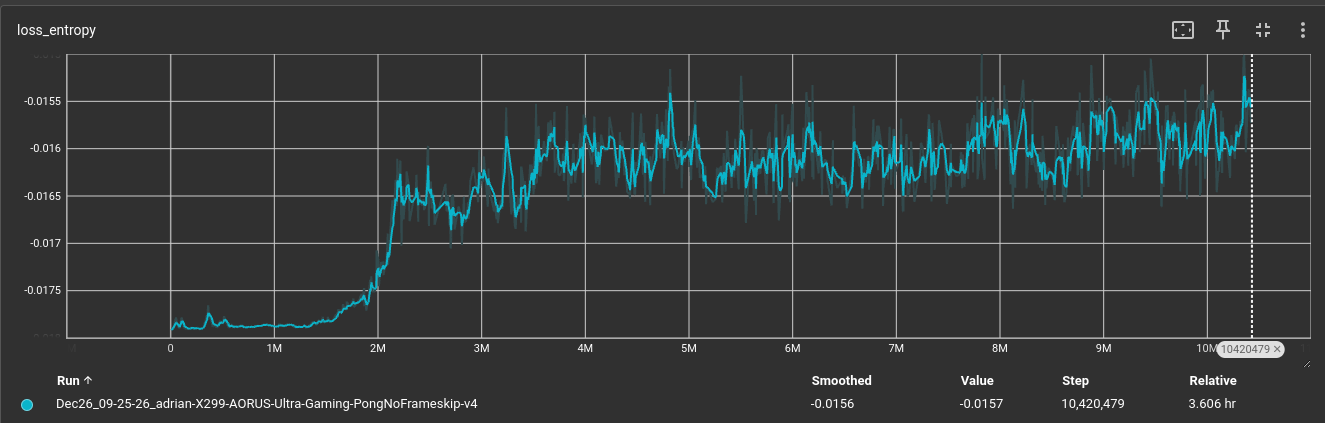
\includegraphics[width=\textwidth]{pictures/A2C_loss_entropy.png}
        \caption{Opis obrazka}
    \end{figure}
    Strata entropii mierzy poziom eksploracji w polityce agenta. Zmniejszająca się wartość entropii w procesie treningu modelu
    oznacza, że model staje się bardziej pewny w procesie podejmowania decyzji. Początkowo wysoka entropia wskazuje na eksplorację,
    następnie jej spadek w późniejszych etapach wskazuje na stabilizację polityki.
    Zasadniczo oznacza to, że podczas gdy polityka zaczyna się zmieniać, agent staje się coraz bardziej pewny akcji, które wykonuje.
    \\ \\ 
    \textbf{Wykres straty polityki}
    \begin{figure}[H]
        \centering
        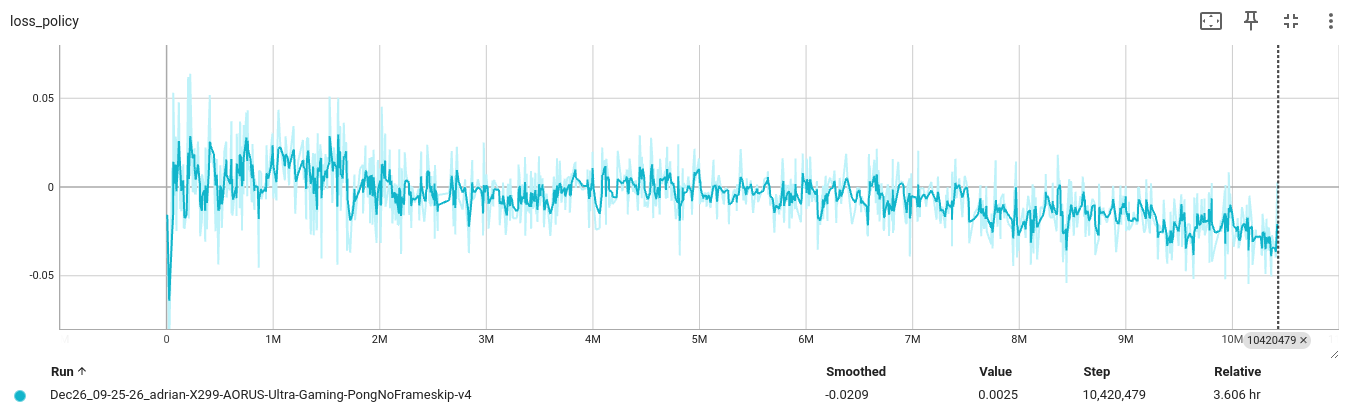
\includegraphics[width=\textwidth]{pictures/A2C_loss_policy.png}
        \caption{Opis obrazka}
    \end{figure}
    Strata polityki pokazuje jak dostosowują się parametry sieci odpowiedzialne za wybór akcji.
    Początkowo zmiaany są intensywne, ale ich stabilizacja w późniejszych etapach treningu wskazuje,
    że agent zbliża się do optymalnej polityki. Generalnie strata plityki zmniejsza się i jest ona skorelowana
    ze stratą całkowitą. Jest to zjawisko pozytywne.
    \\ \\ 
    \textbf{Wykres straty wartości}
    \begin{figure}[H]
        \centering
        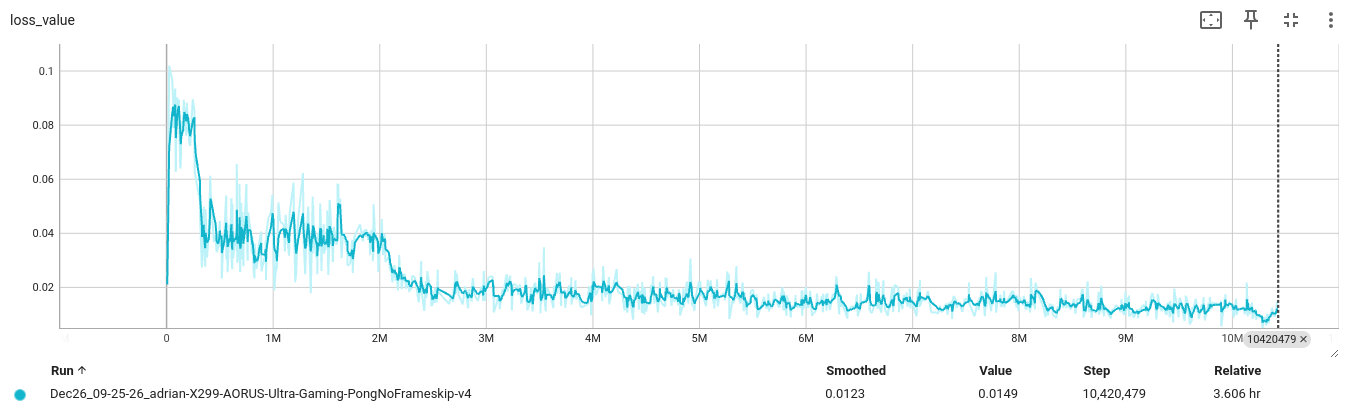
\includegraphics[width=\textwidth]{pictures/A2C_loss_value.png}
        \caption{Opis obrazka}
    \end{figure}
    Strata wartości pokazuje różnicę między przewidywaną a rzeczywistą wartością stanu.
    Konsekwentnie malejąca wartość stanu tej straty podczas procesu treningu oznacza, że przybliżenie \( V(s) \) poprawia się podczas procesu trenowania.
    Wskazuje to na skuteczniejsze podejmowanie decyzji przez model
    \\ \\ 
    \textbf{Wykres całkowitej straty}
    \begin{figure}[H]
        \centering
        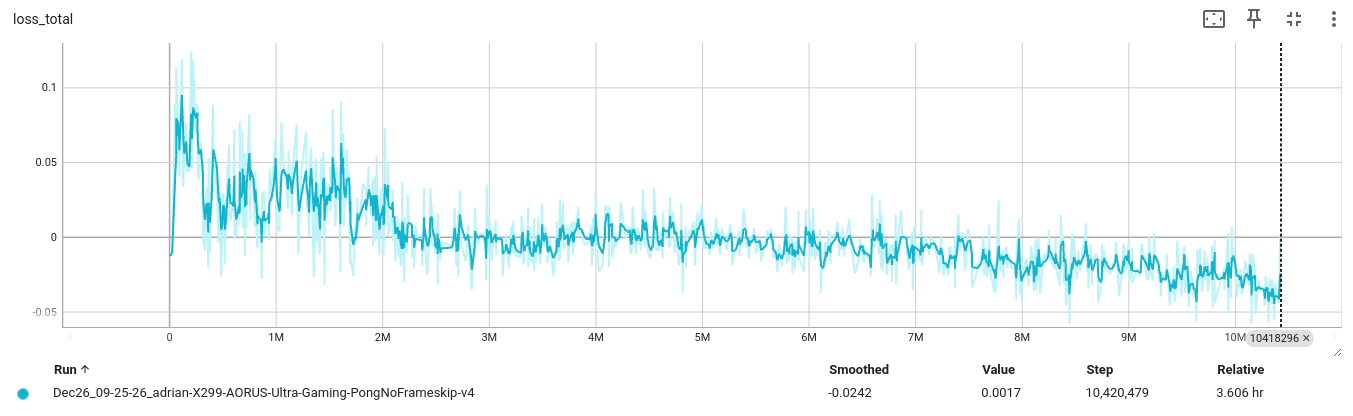
\includegraphics[width=\textwidth]{pictures/A2C_loss_total.png}
        \caption{Opis obrazka}
    \end{figure}
    Łączna strata, która jest sumą strat polityki, wartości oraz entropii.
    Ma zazadanie ona odzwierciedlić ogólny koszt optymalizacji procesu. Całkowita strata systematycznie maleje,
    co pokazuje, że model skutecznie minimalizuje wartość błędu funkcji kosztu.
    Stabilizacja pod koniec procesu uczenia wskazuje na osiągnięcie równowagi między eksploracją a eksploatacją.
    \\ \\ 
    \textbf{Wykres średnich wartości nagród}
    \begin{figure}[H]
        \centering
        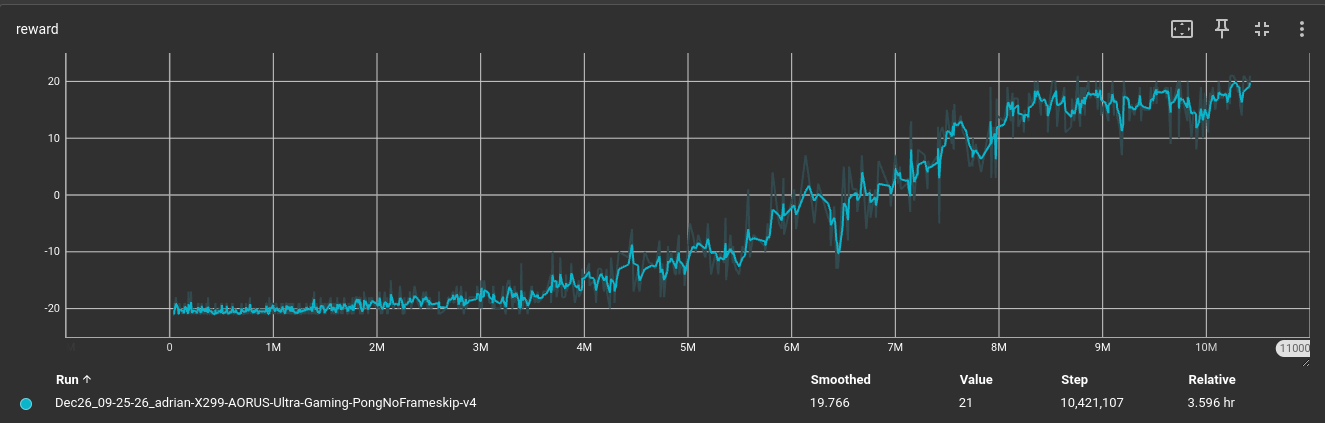
\includegraphics[width=\textwidth]{pictures/A2C_reward.png}
        \caption{Opis obrazka}
    \end{figure}
    Wartość nagrody dla każdego kolejnego epizodu procesu uczenia ilustruje efektywność modelu.
    Początkowe niskie wartości wskazują na fazę eksploracji modelu, a ich systematyczny wzrost sugeruje poprawę strategii wykonywanych przez agenta.
    Średnia nagroda stopniowo rośnie i osiąga maksymalną wartość (około +21), co sugeruje pełne opanowanie środowiska przez agenta.
    \subsubsection{Opis implementacji algorytmu A2C}
    Implementacja modelu składa się z następujących elementów:
    \begin{itemize}
        \item Architektura seici neuronowej - Model A2C składa się z następujących elementów:
        \begin{itemize}
            \item Warstwy konwolucyjne: \textbf{pierwsza warstwa} składa się z 32 filtrów o rozmiarze 8 x 8, kroku 4 oraz funkcji aktywacji ReLU.
            Celem tej warstwy jest wykrycie podstawowych cech obrazu, takich jak krawędzie. 
            \textbf{Druga warstwa} składa się z 64 filtrów o rozmiarze 4 x 4, kroku 2 oraz funkcji aktywacji ReLU.
            Celem tej warstwy jest wydobycie bardziej zaawansowanych cech, takich jak kształty.
            \textbf{Trzecia warstwa} składa się z 64 filtrów o rozmiarze 3 x 3, kroku 1 oraz funkcji aktywacji ReLU.
            Celem tej warstwy jest reprezentacja szczegółowych ceoch obrazu.
            Wyjście z warstw konwolucyjnych jest spłaszczane do jednowymiarowego wektora za pomocą specjalnie napisanej metody,
            która oblicza rozmiar wynikowanego tensoru.
            \item Polityka: odpowiada za generowanie rozkładu prawdopodobieństwa akcji dla danego stanu środowiska. Składa się ona z:
            \textbf{Pierwsza warstwa w pełni połączona}: liczba neuronów 512, funkcja aktywacji ReLu. Celem jest transformacja cech wejściowych
            w bardzeij abstrakcyjne reprezentacje.
            \textbf{Druga warstwa w pełni połączona}: liczba neuronów jest adekwatna do liczby możliwych akcji w środowisku. 
            Funkcja aktywacji liniowa. Celem tej warstwy jest generowanie wartości akcji, które po zastosowaniu funckji softmax przekształcane są na prawdopodobieństwa.
            \item Wartość: estymuje wartości stanu \( V(s) \), czyli oczekiwaną wartość nagordy dla danego stanu. składa się ona z:
            \textbf{Pierwsza warstwa w pełni połączona:} liczba neuronów 512, funkcja aktywacji ReLU. 
            Celem tej warstwy jest ekstrajca cech dla estymacji wartości stanu.
            \textbf{Druga warstwa w pełni połączona:} liczba neuronów 1, fukcja aktywacji liniowa. 
            Celem tej warstwy jest estymacja wartości stanu jako pojedynczej liczby
        \end{itemize}
        \item Mechanizm doświadczeń - 
    \end{itemize}
    \subsubsection{Tabela z wynikami dla różnych hiperparametrów}
    \subsubsection{Wnioski}
    \section{Bibliografia}
    \printbibliography
\end{document} 